\section{Signalizace u krbů}
\begin{figure}[H]
   \centering
    \def\svgwidth{0.3\columnwidth}
    \input{images/svg/otopna-soustava/vyrez-krb-signalizace.pdf_tex}
    \caption[Umístění signalizace u krbu.]{Výřez z obrázku \ref{fig:otopna-soustava-a-elektronika-rez-domu}. Umístění signalizace u krbu.}
    \label{fig:vyrez-krb-signalizace}
\end{figure}

Na obrázku \ref{fig:vyrez-krb-signalizace} je výřez části z celkového nákresu (obrázek \ref{fig:otopna-soustava-a-elektronika-rez-domu}) systému znázorňující umístění signalizace u krbu. Navržená DPS se skládá z části elektronické pojistky TPS2600, zapojení je obdobné jako v \ref{sec:napajeni-1-wire-sbernice} (napájení 1-Wire sběrnice), navíc je na vstupu připojena transilová dioda (ESD9L5.0ST5G). Napěťové meze jsou nastaveny stejně, tedy minimální napětí je 4,75 V, maximální 5,25 V, proud je omezen na maximální hodnotu 100 mA. Dále je zde přivedena 1-Wire sběrnice přes konektor RJ45 s~obdobnými ochranami jako v \ref{sec:datova-cast-1-wire-sbernice} (datová část 1-Wire sběrnice) pro připojení MAX31850K přes svorkovnici. V neposlední řadě jsou zde vstupy pro ovládání třech LED pro signalizaci (obrázek \ref{fig:led-indikace}) naakumulovaného zásobníku otopné vody, modrá LED signalizuje stav horní části zásobníku, oranžová LED je pro střední část, červená je pro signalizaci spodní části. Vstupní část je chráněná přes DS9503 a transilovou diodou (ESD9L5.0ST5G). Sepnutí LED je přes tranzistor (BSS138P). Obdobně jsou řešeny oranžová a modrá LED. Celkové schéma zapojení je v~příloze \ref{app:schemata-ostatni}.

\begin{figure}[H]
    \centering
    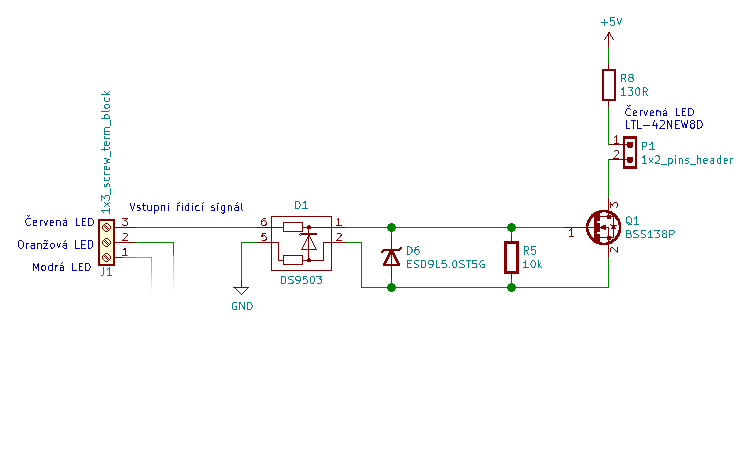
\includegraphics[width=\textwidth]{images/svg/kicad/led-indikace.eps}
    \caption{Zapojení pro ovládání signalizační červené LED.}
    \label{fig:led-indikace}
\end{figure}




\subsubsection{Měření teploty pomocí termočlánku a převodníku MAX31850K}
Teplotní senzory připojené na kouřovody krbů jsou realizované pomocí termočlánku z \ref{sec:teplotni-senzory-pro-krby}. Termočlánek je připojený k zakoupenému modulu (obrázek~\ref{fig:modul-max31850k-1-wire-prevodnik-termoclanku}), hodnota napětí z termočlánku je převedena do digitální podoby včetně teplotní kompenzace studeného konce a~tato hodnota je poslána po 1-Wire sběrnici. Je možné připojit termočlánek typu K. Převodník umožňuje měřit teplotu s~převodem pomocí AD převodníku až na 14 bitů. Rozlišení teploty činí 0,25~°C. Při teplotách -200 °C až 700 °C činí přesnost měřené teploty ±2~°C. Obvod disponuje detekcí zkratu (na GND nebo napájení) na vstupu pro termočlánek. Dále je zde detekce odpojeného termočlánku. Schéma zapojení modulu je v příloze \ref{app:schemata-ostatni}, upraveno z \cite{prevodnik-max31850k}.

%\begin{figure}[H]
%    \centering
%    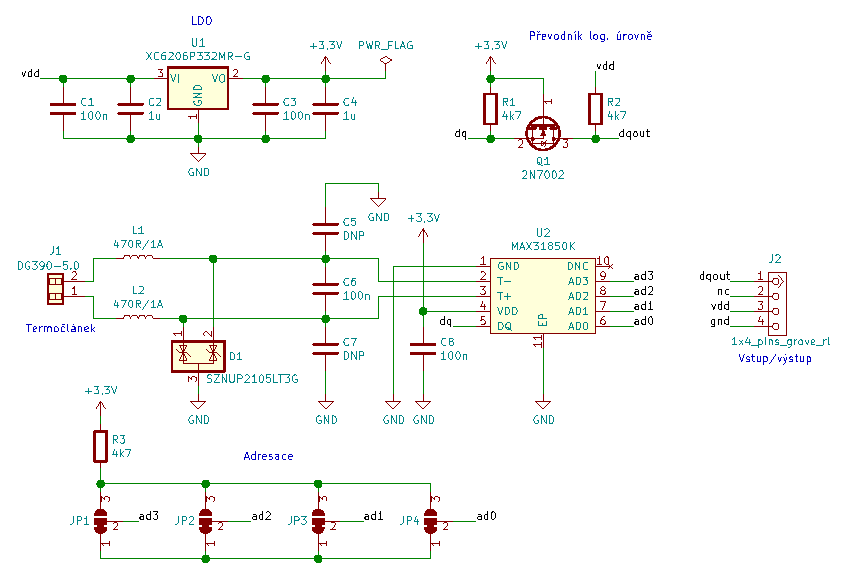
\includegraphics[width=\textwidth]{images/svg/kicad/zapojeni-max31850k-1-wire-prevodnik-termoclanku.eps}
%    \caption[Zapojení MAX31850K v modulu.]{Zapojení MAX31850K v modulu. Upraveno z \cite{prevodnik-max31850k}.}
%    \label{fig:zapojeni-max31850k-1-wire-prevodnik-termoclanku}
%\end{figure}

\begin{figure}[H]
    \centering
    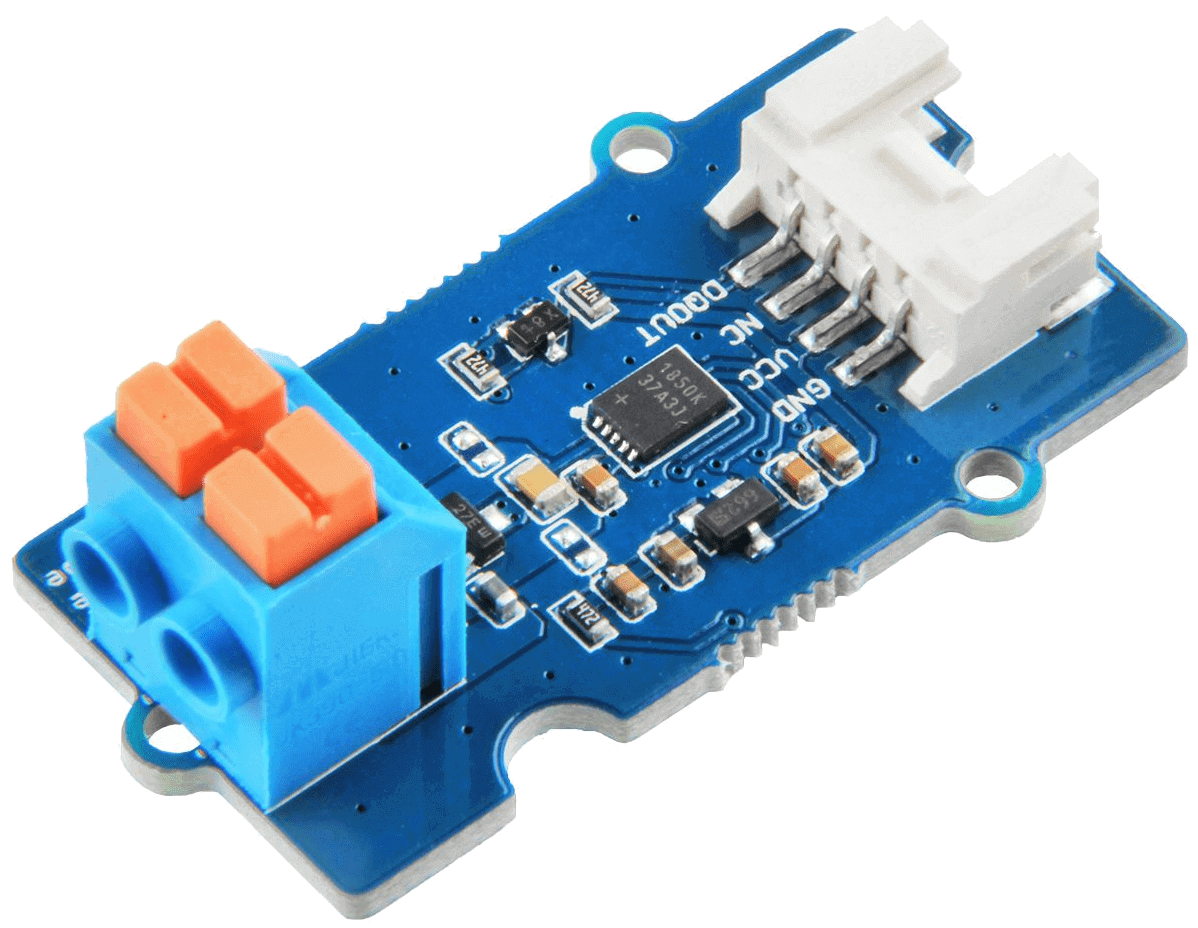
\includegraphics[width=0.4\textwidth]{images/krb/modul-max31850k-1-wire-prevodnik-termoclanku.png}
    \caption[Modul s obvodem MAX31850K.]{Modul s obvodem MAX31850K \cite{prevodnik-max31850k}.}
    \label{fig:modul-max31850k-1-wire-prevodnik-termoclanku}
\end{figure}

\subsubsection{LCD displej}
Pro zobrazování teplot ze střední a spodní části zásobníku otopné vody byl zvolen 16 znakový a 2 řádkový LCD displej s modrým podsvícením a~bílými písmeny (obrázek \ref{fig:lcd-displej}). Pro obsluhu displeje slouží řadič HD44780. K~řadiči je připojen I$^2$C expandér PCF8574 s osmi výstupy, které jsou připojeny na datovou sběrnici pro ovládání respektive zobrazování znaků na displeji. Displej je zapojen za modulem popsaným v části \ref{sec:i2c-sbernice} (I$^2$C sběrnice). Každý displej, respektive expandér PCF8574 umožňuje nastavit pomocí propojek A0, A1, A2 unikátní adresu zařízení na sběrnici.

\begin{figure}[H]
\centering
\begin{subfigure}{.5\textwidth}
  \centering
  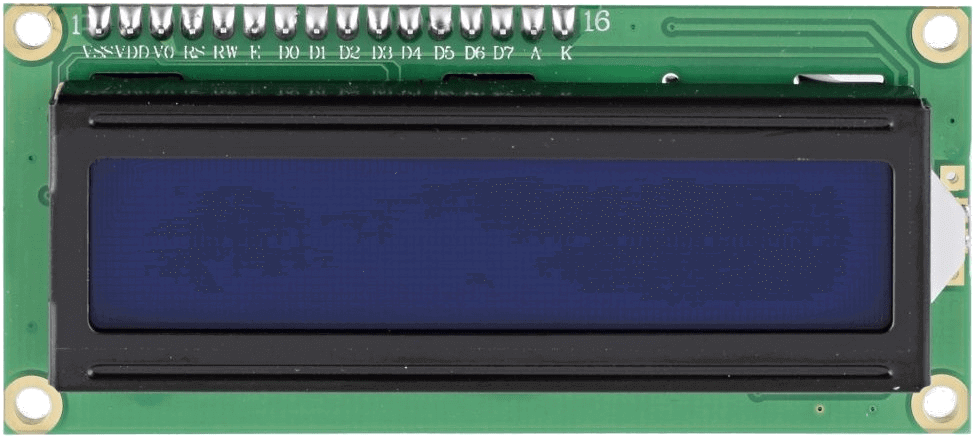
\includegraphics[width=0.91\linewidth]{images/krb/predni-cast-lcd-displeje.png}
  \caption{Přední část displeje.}
  \label{fig:predni-cast-lcd-displeje}
\end{subfigure}%
\begin{subfigure}{.5\textwidth}
  \centering
  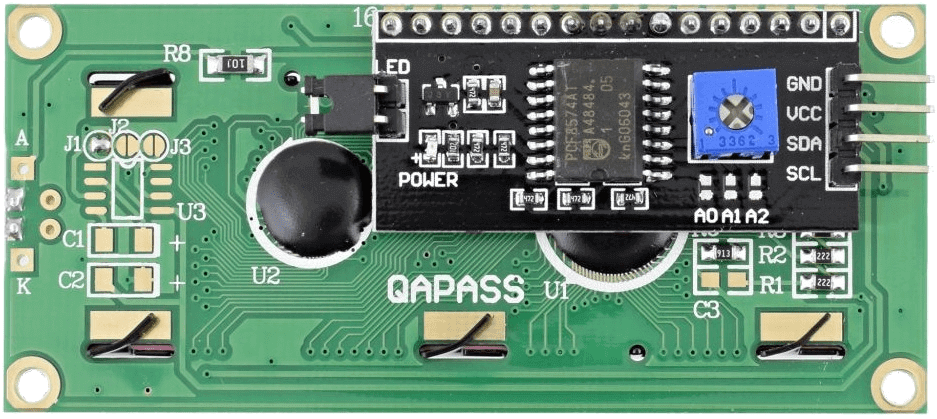
\includegraphics[width=0.9\linewidth]{images/krb/zadni-cast-lcd-displeje-s-expanderem-pcf8574.png}
  \caption{Zadní část displeje s I$^2$C expandérem PCF8574.}
  \label{fig:zadni-cast-lcd-displeje-s-expanderem-pcf857}
\end{subfigure}
\caption[LCD displej pro zobrazování teplot ze zásobníku otopné vody.]{LCD displej pro zobrazování teplot ze zásobníku otopné vody \cite{lcd-displej}.}
\label{fig:lcd-displej}
\end{figure}

\subsubsection{Realizovaná DPS signalizace u krbů}
Výše popsané části jsou realizované na DPS (obrázek \ref{fig:dps-led-ochrany-u-krbu-spodek}, \ref{fig:dps-led-ochrany-u-krbu-vrsek}, \ref{fig:dps-led-ochrany-u-krbu-kabely}). Deska byla vlastnoručně navržena, vyrobena a osazena. Je aplikován ochranný lak. Celkové schéma zapojení je v příloze \ref{app:schemata-ostatni}.

\begin{figure}[H]
    \centering
    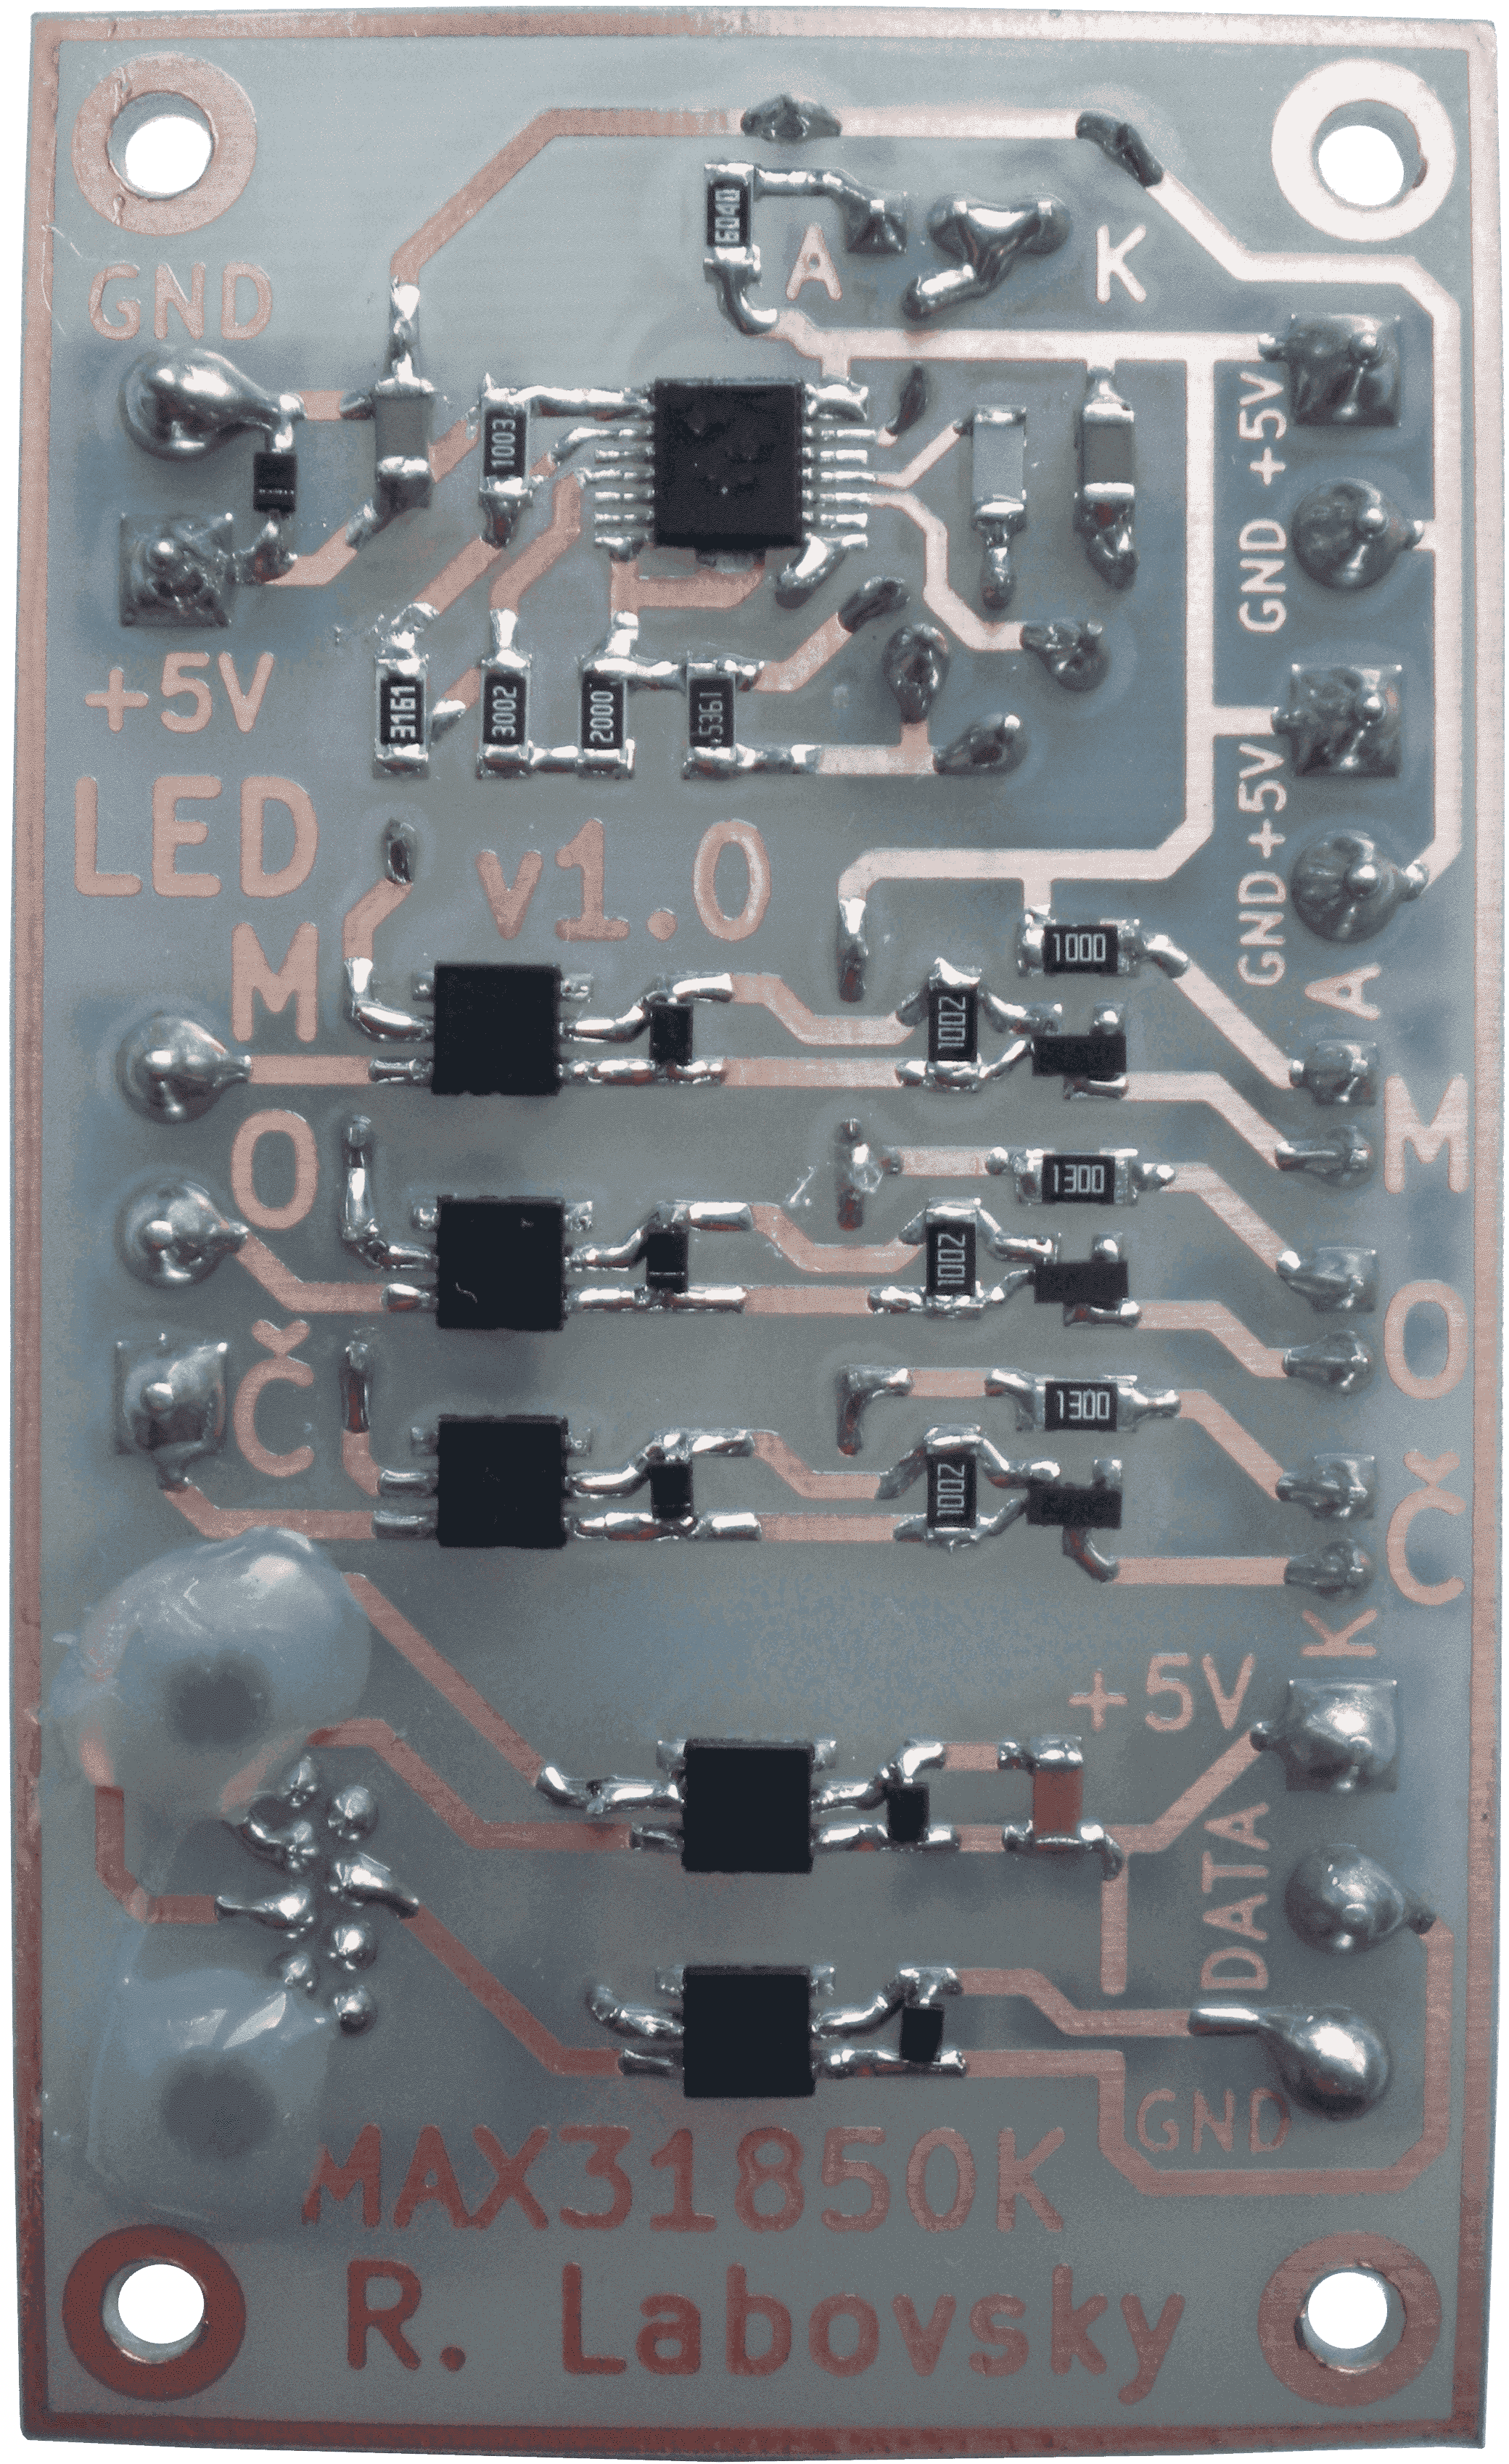
\includegraphics[width=0.8\textwidth]{images/krb/dps-led-ochrany-u-krbu-spodek.png}
    \caption{Spodní část DPS pro signalizaci u krbu.}
    \label{fig:dps-led-ochrany-u-krbu-spodek}
\end{figure}

\begin{figure}[H]
    \centering
    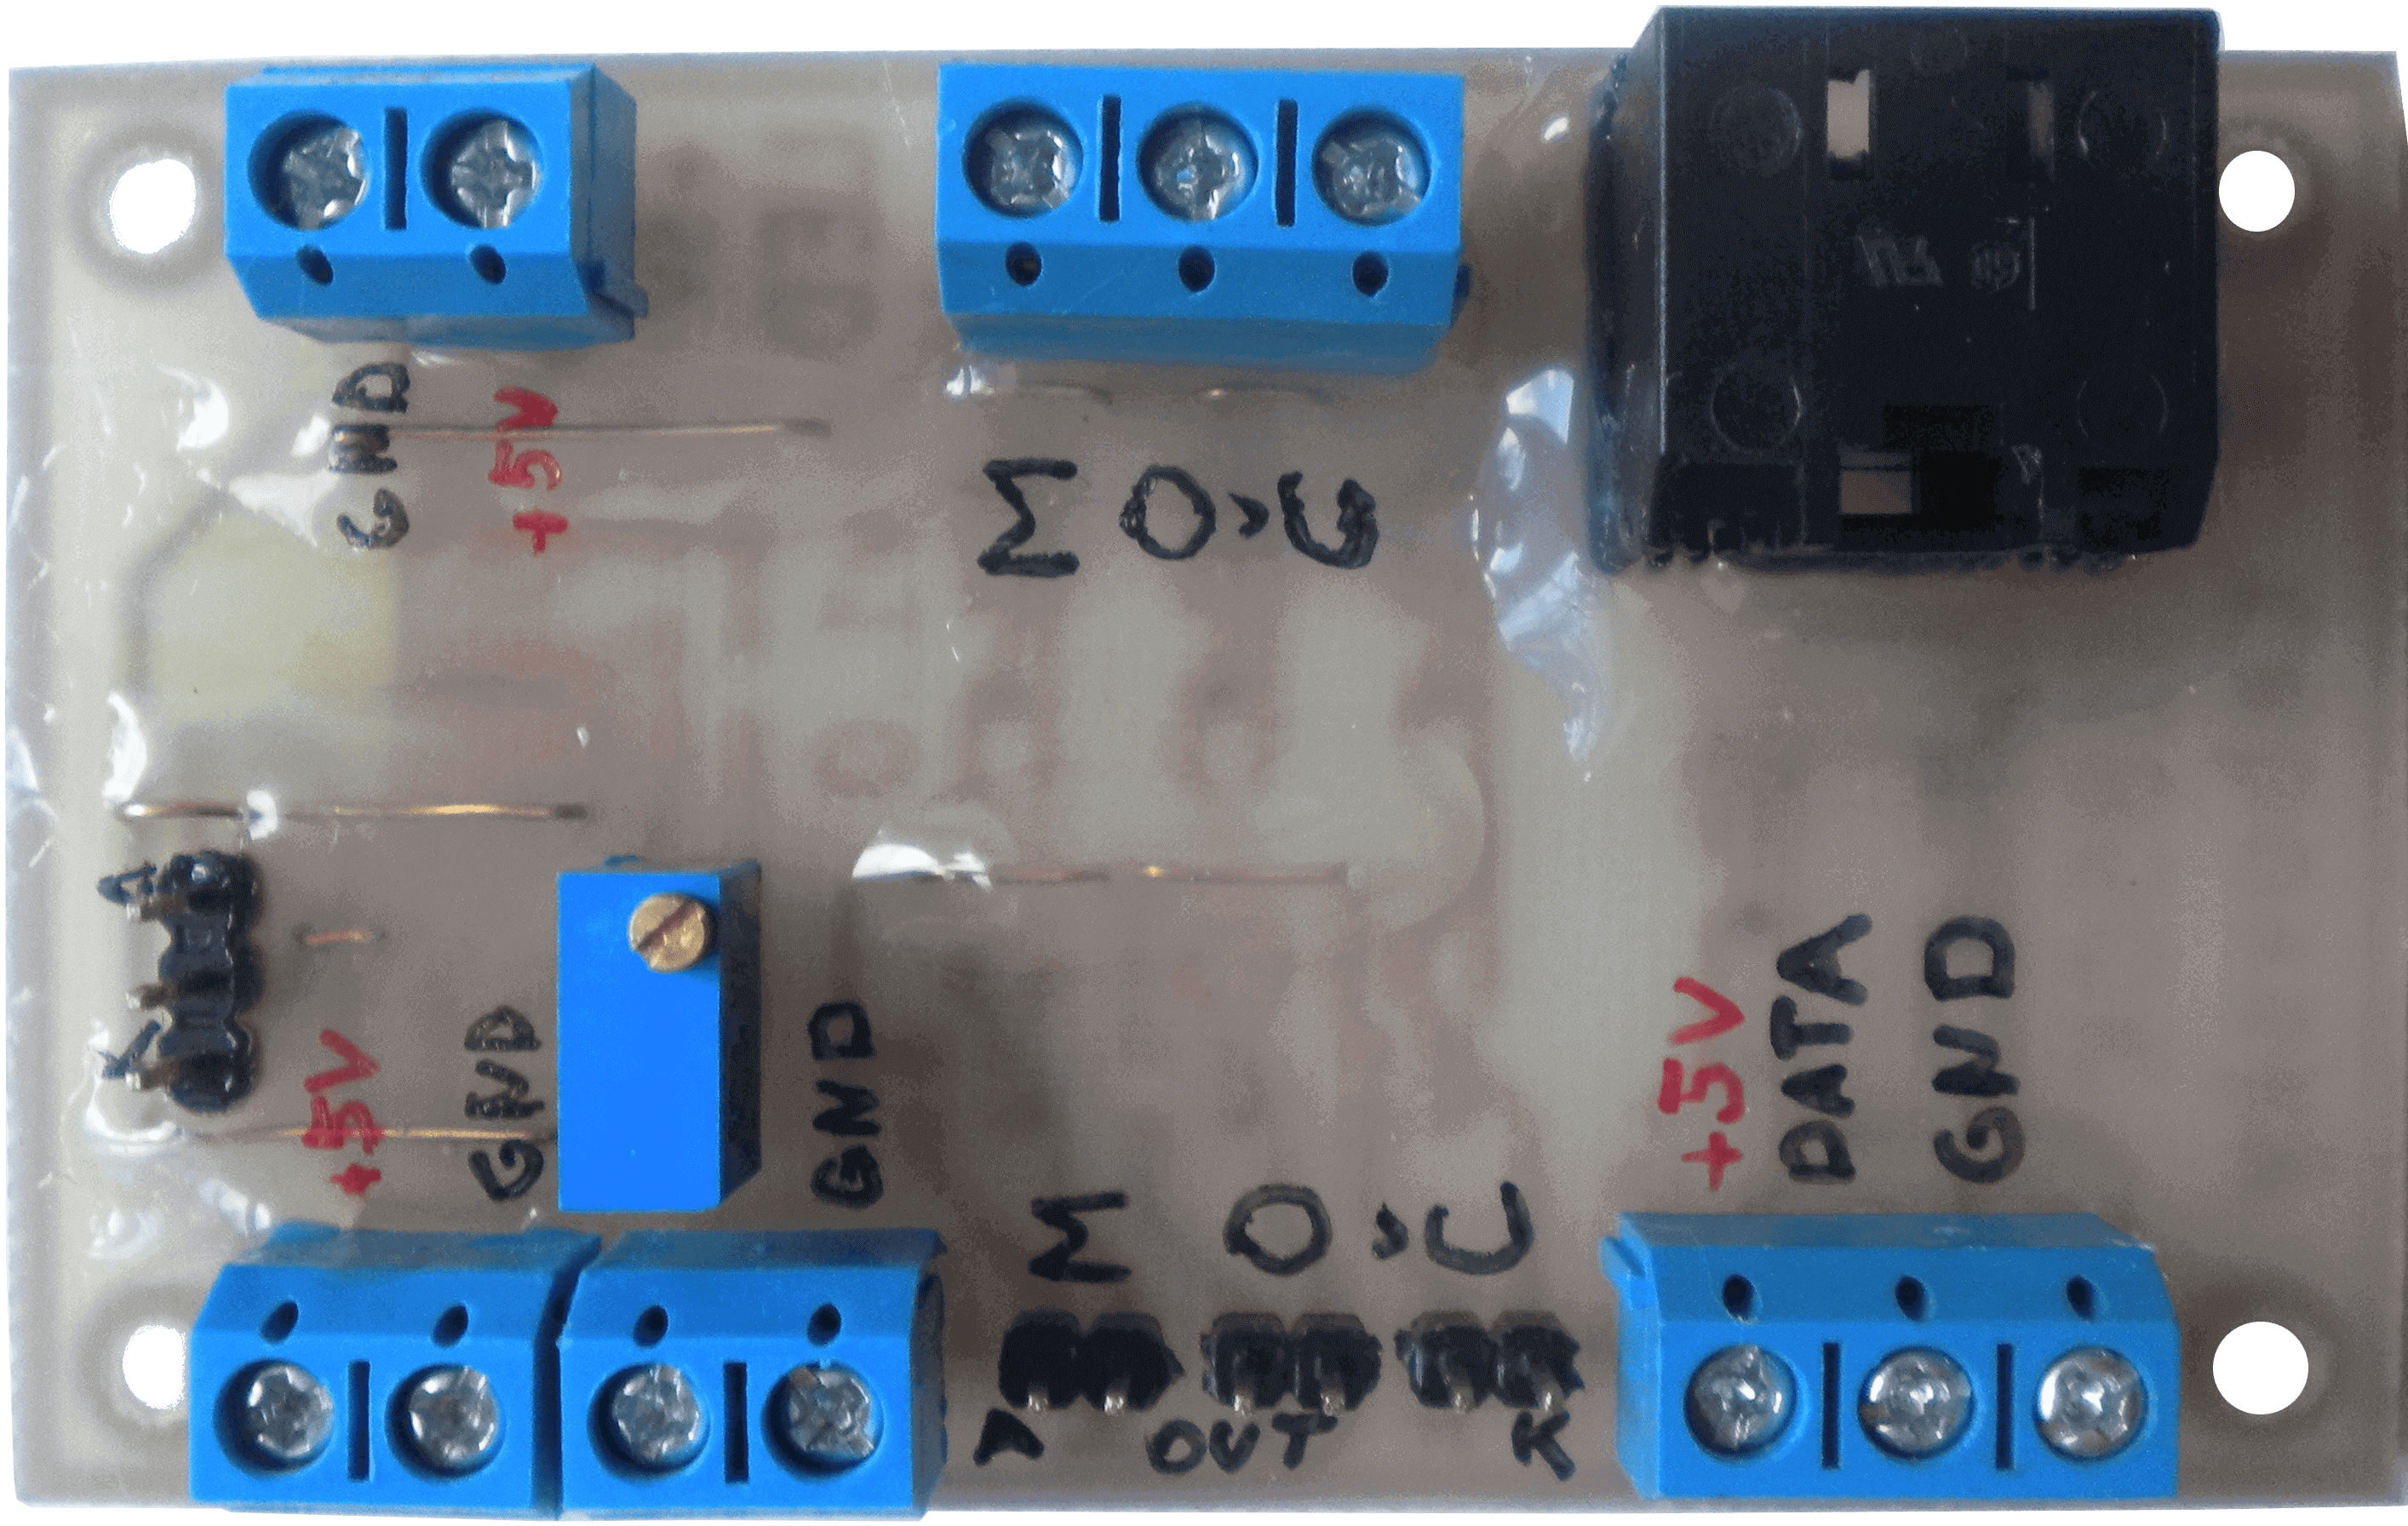
\includegraphics[width=0.8\textwidth]{images/krb/dps-led-ochrany-u-krbu-vrsek.png}
    \caption{Horní část DPS pro signalizaci u krbu.}
    \label{fig:dps-led-ochrany-u-krbu-vrsek}
\end{figure}

\begin{figure}[H]
    \centering
    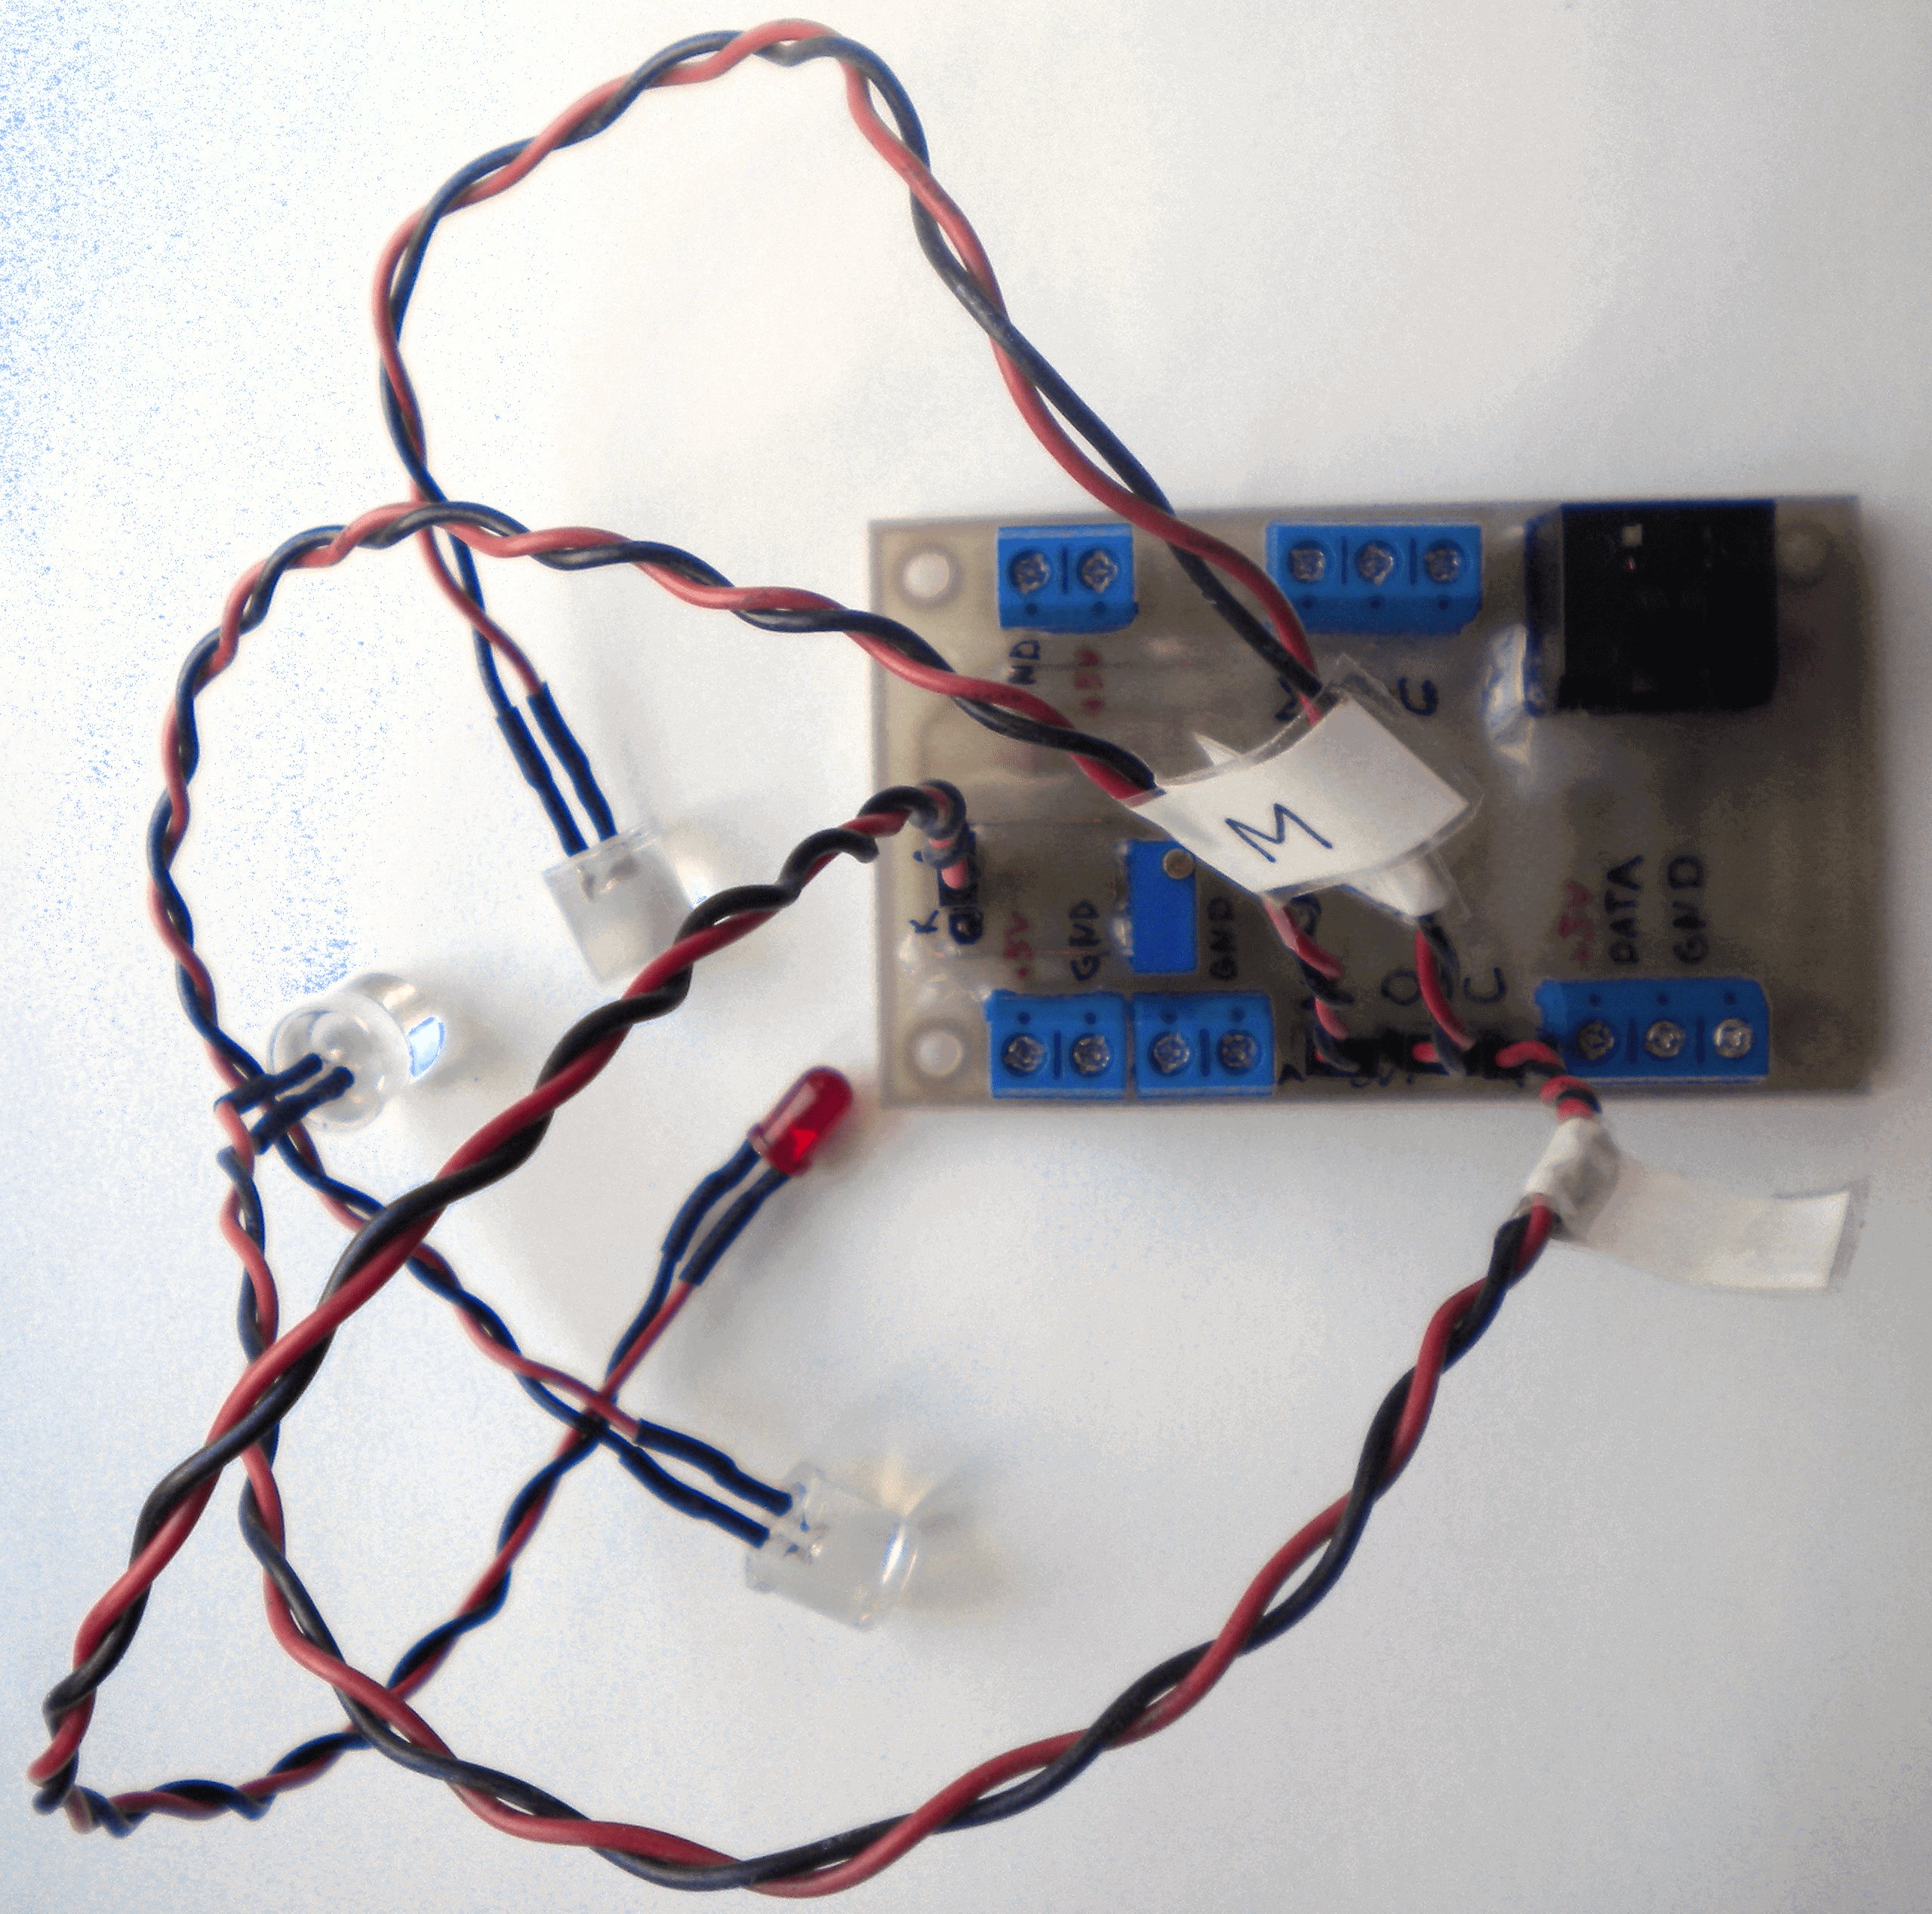
\includegraphics[width=0.8\textwidth]{images/krb/dps-led-ochrany-u-krbu-kabely.png}
    \caption{DPS včetně signalizačních LED.}
    \label{fig:dps-led-ochrany-u-krbu-kabely}
\end{figure}

\subsubsection{Instalační krabice}
Všechna elektronika je umístěna do ochranné instalační krabice (obrázek \ref{fig:instalacni-krabice-vnitrek-krb}). Do krabice vstupují dva vodiče pro napětí 5 V a zem, tři kabely pro ovládání signalizačních LED, UTP kabel se sběrnicí 1-Wire pro teplotní senzor (termočlánek) a I$^2$C sběrnicí. Na obrázku \ref{fig:zadni-cast-krytu-vika-instalacni-krabice-krb} je zobrazena zadní část víka instalační krabice s uchycením signalizačních LED a LCD displeje. Na obrázku \ref{fig:predni-cast-krytu-vika-instalacni-krabice-krb} je přední část víka instalační krabice. Takto zkompletovaná instalační krabice je umístěna u krbu ve sklepě, v přízemí a v patře.

%\begin{figure}[H]
%    \centering
%    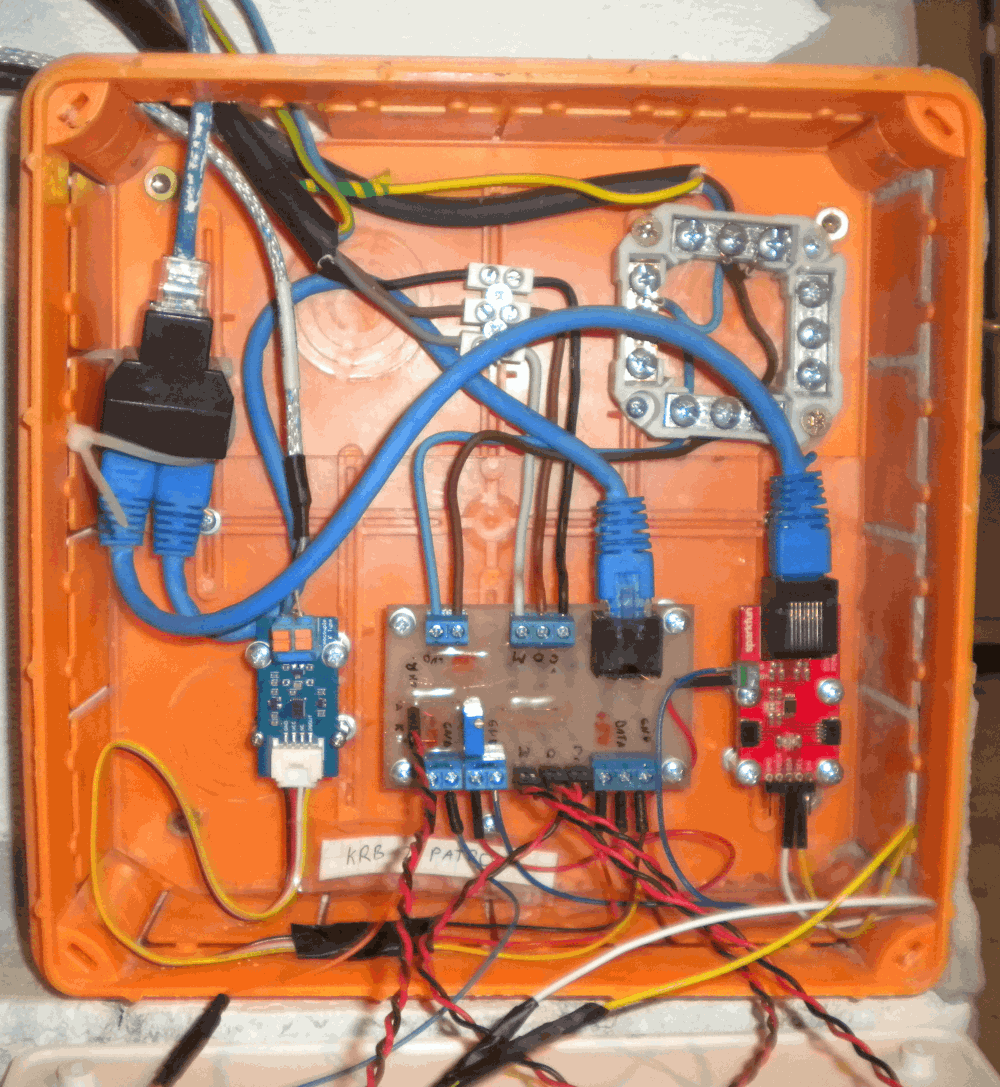
\includegraphics[width=0.6\textwidth]{images/krb/instalacni-krabice-vnitrek-krb.png}
%    \caption{Instalační krabice s jednotlivými moduly.}
%    \label{fig:instalacni-krabice-vnitrek-krb}
%\end{figure}

%\begin{figure}[H]
%    \centering
%    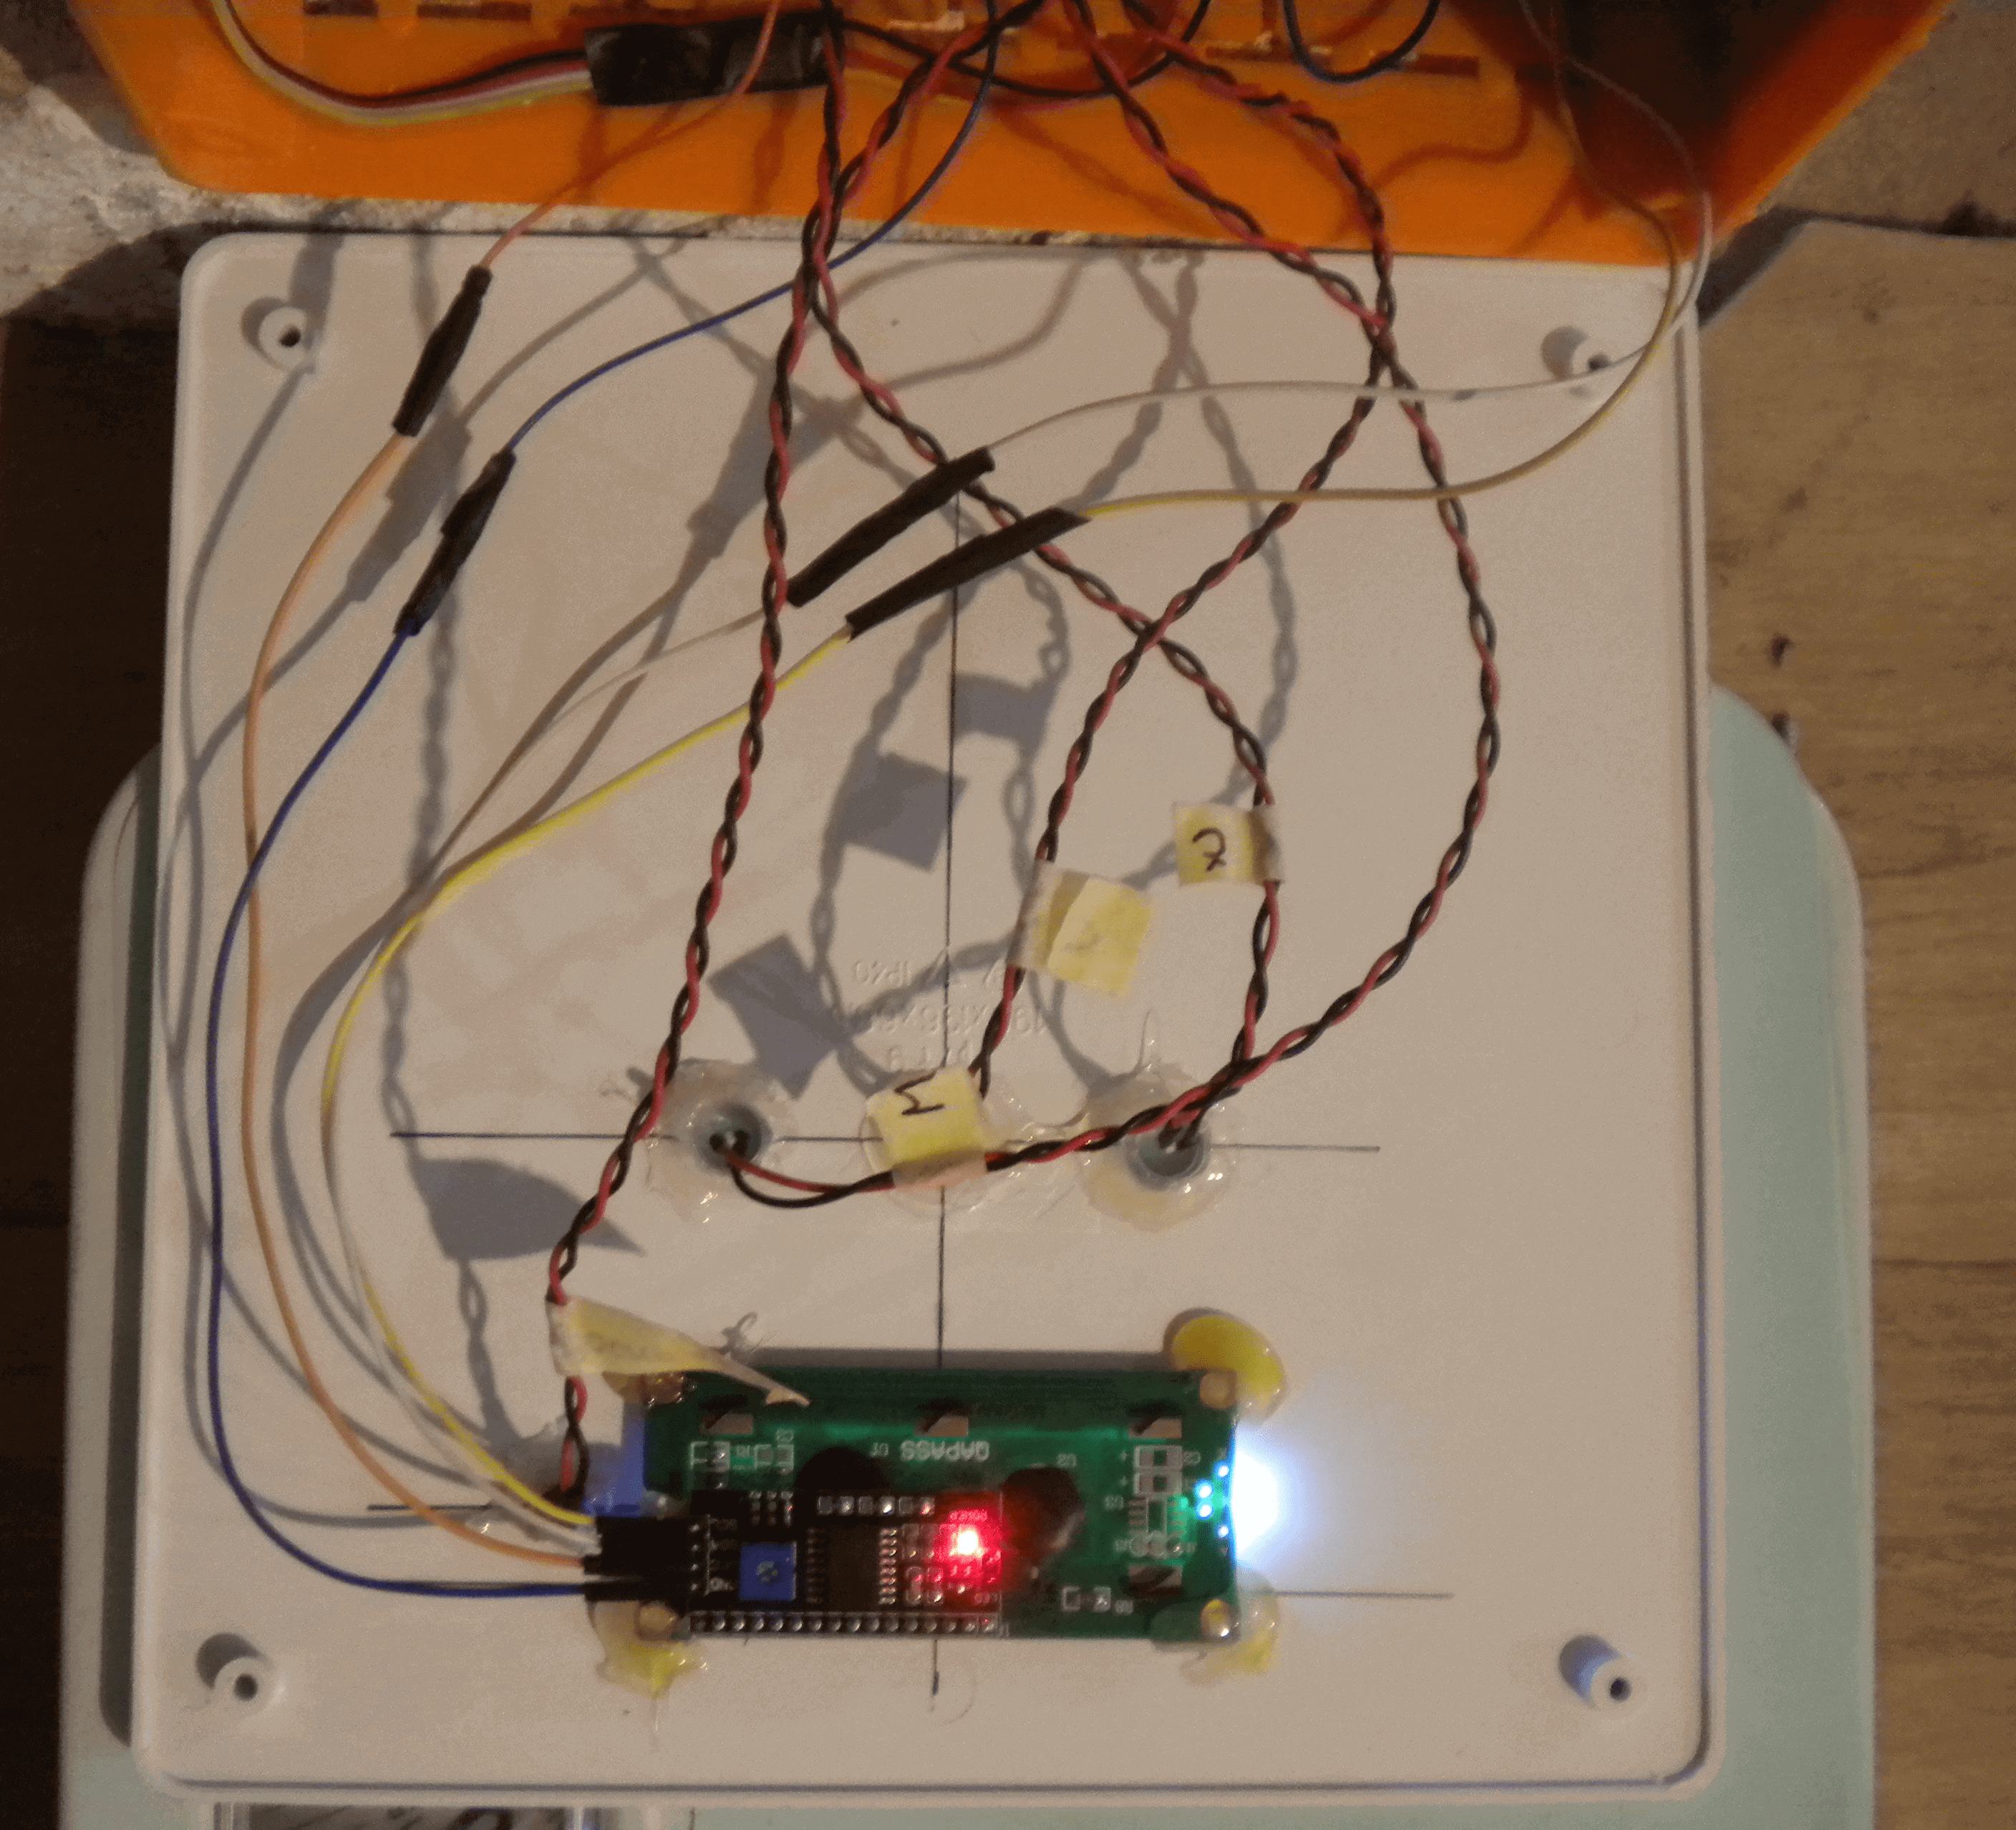
\includegraphics[width=0.6\textwidth]{images/krb/zadni-cast-krytu-vika-instalacni-krabice-krb.png}
%    \caption{Zadní část instalační krabice.}
%    \label{fig:zadni-cast-krytu-vika-instalacni-krabice-krb}
%\end{figure}



\begin{figure}[H]
\centering
\begin{subfigure}{.5\textwidth}
  \centering
  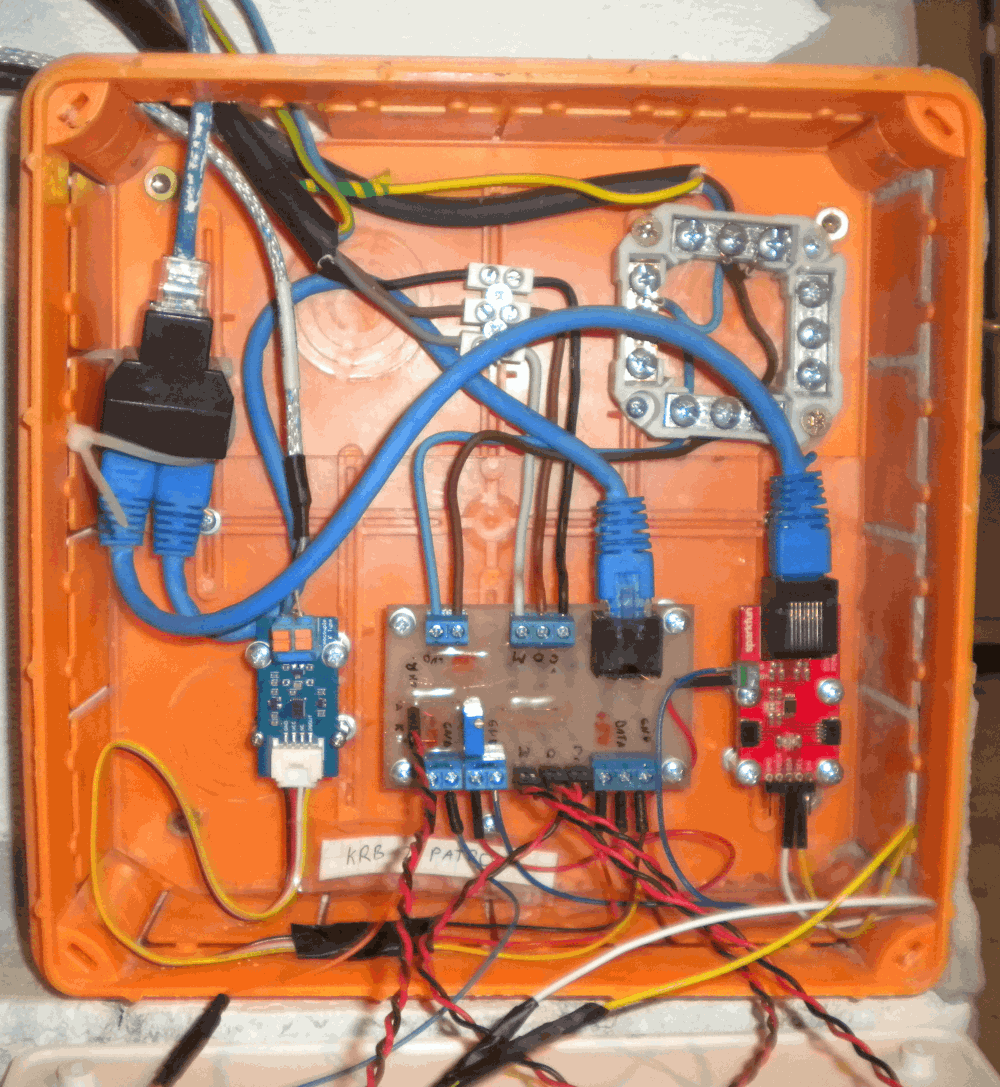
\includegraphics[width=0.835\textwidth]{images/krb/instalacni-krabice-vnitrek-krb.png}
  \caption{Instalační krabice s jednotlivými moduly.}
  \label{fig:instalacni-krabice-vnitrek-krb}
\end{subfigure}%
\begin{subfigure}{.5\textwidth}
  \centering
  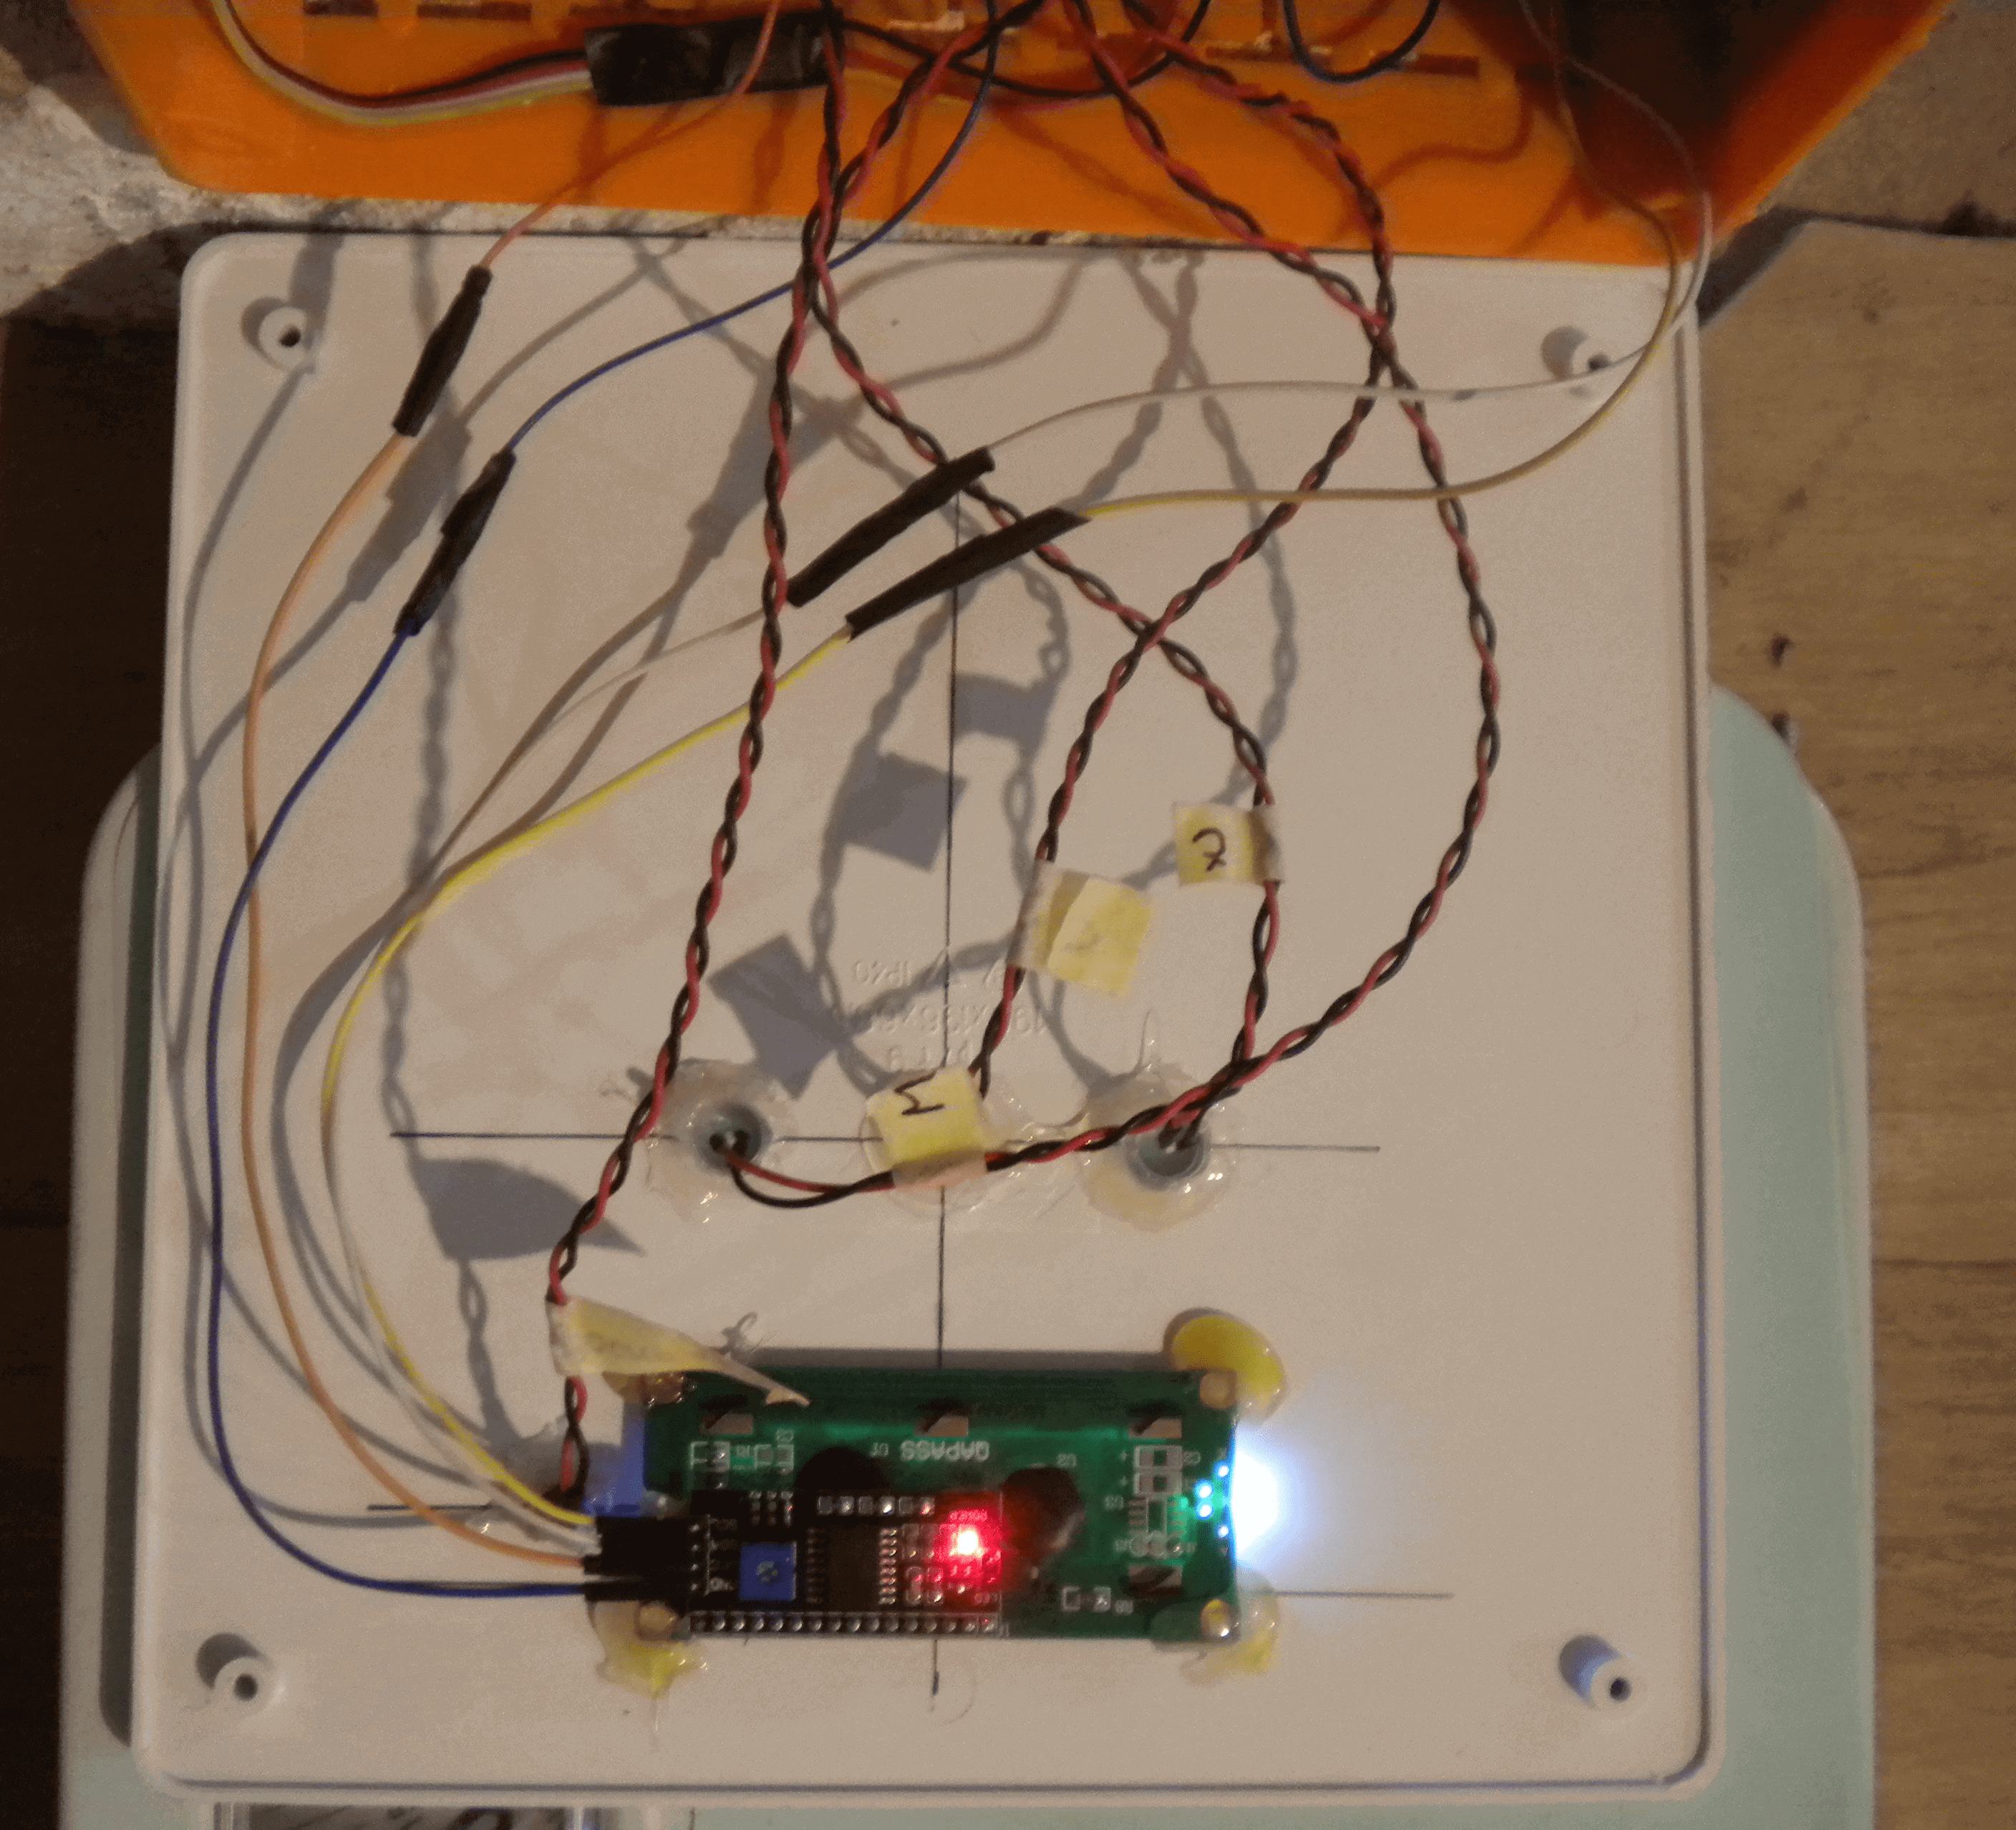
\includegraphics[width=\textwidth]{images/krb/zadni-cast-krytu-vika-instalacni-krabice-krb.png}
  \caption{Zadní část instalační krabice.}
  \label{fig:zadni-cast-krytu-vika-instalacni-krabice-krb}
\end{subfigure}
\caption{Instalační krabice pro signalizaci.}
\label{fig:instalacni-krabice}
\end{figure}



\begin{figure}[H]
    \centering
    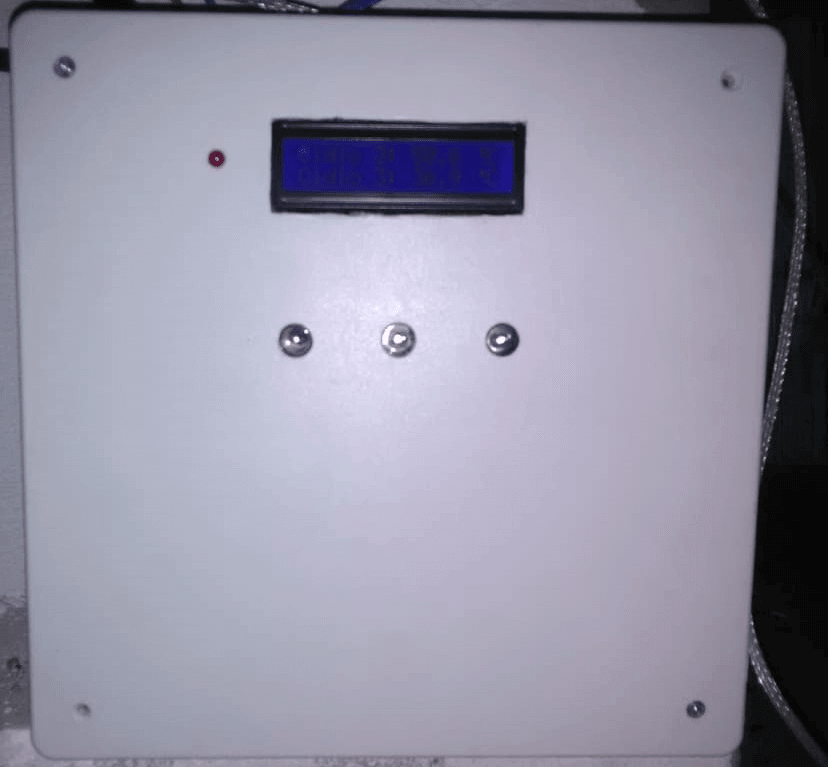
\includegraphics[width=0.55\textwidth]{images/krb/predni-cast-krytu-vika-instalacni-krabice-krb.png}
    \caption[Víko instalační krabice.]{Víko instalační krabice. Osazený LCD displej, signalizačních LED (zleva modrá, oranžová a červená) a LED pro aktivování elektronické pojistky (červená LED vlevo od displeje).}
    \label{fig:predni-cast-krytu-vika-instalacni-krabice-krb}
\end{figure}


